\subsection{Block with pressure problem}
The incompressible block problem shown in Figure \ref{fg:block_model} is considered for testing 3D mixed formulations,
the block's dimensions are $2L\times 2L \times L$, $L=1$. At the center of the top surface of the block is applied a pressure load $P = 1$ with the area of $L\times L$.
Due to the symmetry of this problem, only quarter model is considered.
The Young's modulus and Poisson's ratio are set as $E = 3\times 10^6$ and $\nu = 0.5-10^{-8}$, respectively.

\begin{figure}[H]
\centering
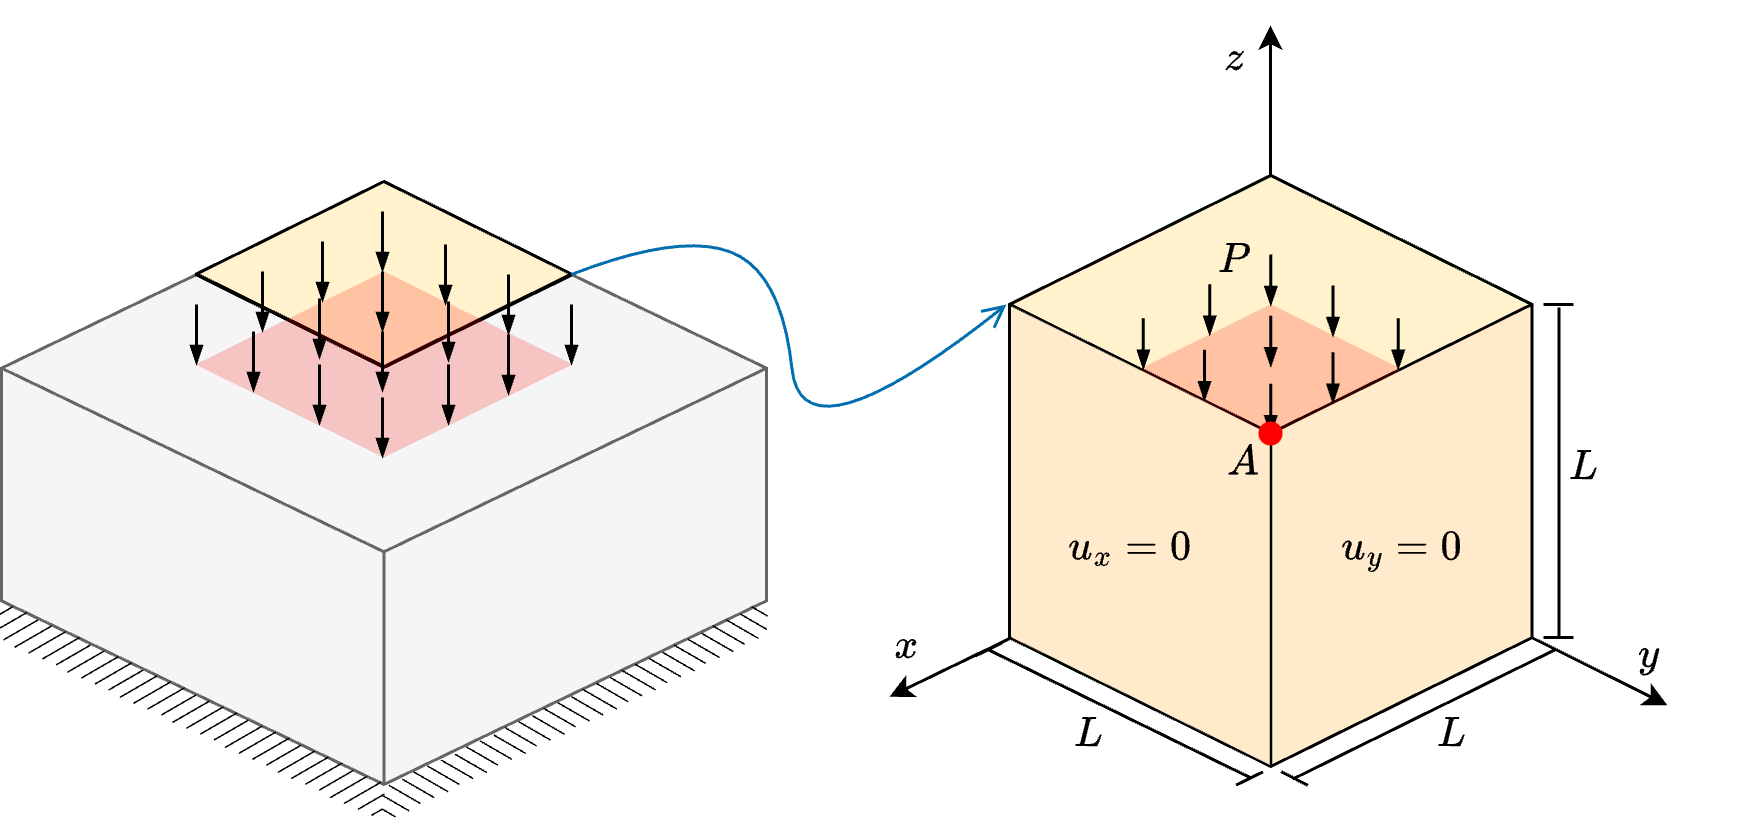
\includegraphics[width=\textwidth]{png/block.png}
\caption{Illustration of block under compression problem}\label{fg:block_model}
\end{figure}

Figures study the pressure stability of 3D mixed FE-meshfree formulations, Tet4--RK and Hex8--RK, with non--uniform nodal distribution, while the pressure discretized by linear meshfree approximations with characterized support size of 1.5.
The corresponding results also show the well performance of the proposed optimal constraint ratio $r=r_{opt}$.
The mixed formulations with traditional constraint ratio $r=n_d$ show a comparable displacement results, but exhibit a significant pressure instability.
